\documentclass[12pt]{article}

\usepackage{graphicx,amssymb,amsmath,subfig,amsfonts}
\usepackage{url}
\usepackage{natbib}
\usepackage{hyperref}
\usepackage{cleveref}%to have automatic 'clever' references that includes the words 'figure', 'equation', etc.


\linespread{1.3}



%%%%%%%%%%%%%%%%%%%%%%%%%%%%%%%%%%%%%
\newcommand{\ud}{\mathrm{d}}
\newcommand{\e}{\text{e}}
\newcommand{\mtx}[1]{\mathbf{ #1}}
\newcommand{\E}[1]{{\mathrm E}\left[ #1 \right]}
\newcommand{\Var}[1]{{\mathrm Var}\left[ #1 \right]}
\newcommand{\Cov}[1]{{\mathrm Cov}\left[ #1 \right]}



% ------
% Maketitle metadata
\title{\vspace{-15mm}%
	\fontsize{24pt}{10pt}\selectfont
	\textbf{Math behind Country\--Capability\--Product Decomposition}
	}	
\author{%
	\large
	\textsc{Andres Gomez-Lievano} \\[1.5mm]
	\normalsize	Center for International Development, HKS, Harvard University %\\
	%\normalsize	\href{mailto:andres\_gomez@hks.harvard.edu}{andres\_gomez@hks.harvard.edu}
	\vspace{-5mm}
	}
\date{}


%%%%%%%%%%%%%%%%%%%%%%%%
\begin{document}

\maketitle



\section{Statement of the Problem}
Our starting point is the empirical matrix $\mtx{M}$ that identifies the products that countries export with a relative comparative advantage:
$$
[\mtx{M}]_{c,p}=1,\quad\text{if $RCA_{c,p}>1$}.
$$

The empirical matrix we observe whereby some countries are able to produce some products we hypothesize comes from an interaction between a matrix $\mtx{C_{ca}}$ of countries and different capabilities they may have, and another matrix $\mtx{P_{ap}}$ specifying the capabilities that products require to get produced. The problem is to infer these two matrices from $\mtx{M}$ plus a minimum number of assumptions.

\section{Framework: Stochastic Matrices}
Before we tackle directly our problem, let us show that we can manipulate more easily our matrices if we represent them as stochastic matrices. The reason for this is that the product of stochastic matrices is still a stochastic matrix. And stochastic matrices work, from a certain point of view, as matrices that translate a state of the world into another. 

Let us consider the bipartite network representing $\mtx{M}$, which connects countries with products. And let us consider a random walker in this network. Suppose there is a probability $\pi_p(t)$ that the random walker is in product $p$ at time $t$. The probability that the random walker will end up at country $c$ at $t+1$ (after randomly following one of the edges on the bipartite network) can be expressed as:
\begin{align}
	\Pr\{&~\text{ending at $c$ at $t+1$}~\} \nonumber\\
	=& \sum_{p}\Pr\{~\text{ending at $c$ at $t+1$}~|~\text{starting at $p$ at $t$}~\}~\Pr\{~\text{starting at $p$ at $t$}~\}.\nonumber
\end{align}

In terms of our matrix $\mtx{M}$, and given the vector $\vec{\pi}(t)$ of starting in any of the products, the previous equation becomes
\begin{align}
	\gamma_c(t+1) = \sum_{p}\left(\frac{M_{c,p}}{\sum_{c'} M_{c',p}}\right)\pi_p(t),
\end{align}
where $\vec{\gamma}(t+1)$ is the vector of probabilities of being in the different countries at the time-step $t+1$. In matrix notation, we write this as
\begin{equation}
	\vec{\gamma}(t+1) = \mtx{Q}_{c\leftarrow p}\cdot\vec{\pi}(t).
\label{eq:p2c}
\end{equation}
I have explicitly specified that the stochastic matrix $\mtx{Q}$ is a transition matrix from products to countries (i.e., ``$c\leftarrow p$''), and is thus a \emph{left-stochastic} matrix\footnote{A left-stochastic matrix has the property that its columns add up to 1. We transition from states and their probabilities to future states by multiplying on the right by a vector of probabilities for the previous states.}. 

We can do a similar exercise but starting from countries and ending up at products. This yields
\begin{equation}
	\vec{\pi}^T(t+1) = \vec{\gamma}^T(t)\cdot\mtx{R}_{c\rightarrow p},
\label{eq:c2p}
\end{equation}
where $(\cdot)^T$ is the transpose operation, $\mtx{R}$ is the transition matrix that takes me from countries to products (i.e., ``$c\rightarrow p$''), and is thus a \emph{right-stochastic} matrix:
$$
\mtx{R}_{c\rightarrow p}=\left(\frac{M_{c,p}}{\sum_{p'} M_{c,p'}}\right).
$$

Transition matrices $\mtx{Q}_{c\leftarrow p}$ and $\mtx{R}_{c\rightarrow p}$ can be expressed explicitly in terms of $\mtx{M}$ as
\begin{align}
	\mtx{Q} &= \mtx{M}\cdot \text{diag}(\vec{1}^T\cdot\mtx{M})^{-1},\\
	\mtx{R} &= \text{diag}(\mtx{M}\cdot\vec{1})^{-1}\cdot\mtx{M},	
\end{align}
where the function $\text{diag}(\vec{x})$ takes the elements of the vector $\vec{x}$ and puts them into the diagonal of a square matrix.

\subsection{The Product Space}
We note that we can transition from products to countries, and back from countries to products. thus, the transition matrix that takes me from products to products is the multiplication of $\mtx{R}^T$ and $\mtx{Q}$:
\begin{align}
	\vec{\pi}(t+2) &= \mtx{R}^T\cdot\vec{\gamma}(t+1),\quad\text{(transposing \cref{eq:c2p})}\\
	&= \mtx{R}^T\cdot\mtx{Q}\cdot\vec{\pi}(t),\quad\text{(using \cref{eq:p2c})}.
\label{eq:p2p}
\end{align}

Hence, the transition left-stochastic matrix that takes me from products to products is
$$
	\mtx{S_{pp}} = \mtx{R}^T\cdot\mtx{Q}.
$$
This matrix \emph{is} the Product Space. Note, for instance, that the \emph{dominant right-eigenvector} (corresponding to the eigenvalue $\lambda_1=1$) of $\mtx{S_{pp}}$ is the stationary distribution of the random walker at $t\rightarrow\infty$, such that $\vec{\pi}_{\infty}=\mtx{S_{pp}}\vec{\pi}_{\infty}$ (sometimes called the perron-vector).

Note that the Country Space can be constructed in a similar way, yielding
$$
	\mtx{S_{cc}} = \mtx{Q}\cdot\mtx{R}^T.
$$

\subsubsection{Commentary on Complexity Indices}
Notice that our complexity indices are defined such that:
\begin{align}
	\vec{pci}^T\cdot \mtx{S_{pp}} = \lambda^{(products)}_2\vec{pci}^T , 
\end{align}
and
\begin{align}
	\vec{eci}^T\cdot \mtx{S_{cc}} = \lambda^{(countries)}_2\vec{eci}^T,
\end{align}
where $\lambda^{(products)}_2$ and $\lambda^{(countries)}_2$ are the \emph{sub-dominant} eigenvalues of the product and country spaces, respectively.

\section{The solution to our problem}
\begin{figure}[!ht]
		\centering
			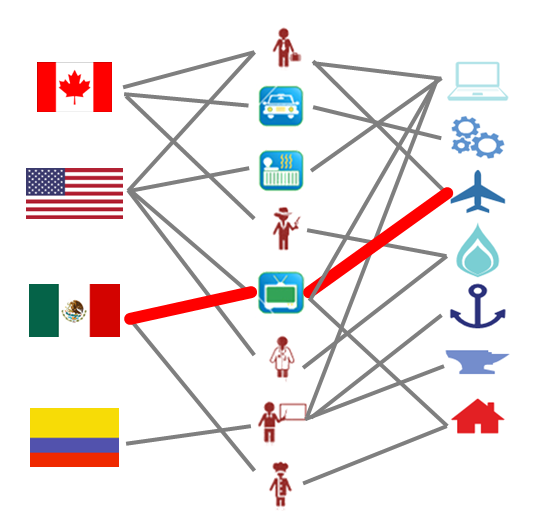
\includegraphics[width=0.5\linewidth]{CAP.png}
		\caption{The networks that connect countries with capabilities, and capabilities to products, can be re-expressed as stochastic matrices. Since the product of stochastic matrices is still a stochastic matrix, factorization may be possible.
		}
\label{fig:cap}
\end{figure}

\subsection{Expressing our matrices properly}
Assume now that between countries and products there is an intermediate step made of capabilities (see \cref{fig:cap}). A random walker in this expanded network will transition, for example, from products to capabilities, and from capabilities to countries. The product space, in this case, will be defined by a transition of the form: $p'\rightarrow a\rightarrow c\rightarrow a \rightarrow p$, where $a$ denotes a single capability $a$ (with $a=1,\ldots, N_\alpha$). The product space is thus a multiplication of four transition matrices.

The transition matrix $\mtx{R}$ from countries to products can now be expressed in terms of $\mtx{C_{ca}}$ and $\mtx{P_{ap}}$ matrices as:
\begin{align}
	\mtx{R}&=\left( \text{diag}(\mtx{C_{ca}}\cdot\vec{1})^{-1}\cdot\mtx{C_{ca}} \right)\cdot\left( \text{diag}(\mtx{P_{ap}}\cdot\vec{1})^{-1}\cdot\mtx{P_{ap}} \right)\\
	&=\left( \mtx{{}_C\Delta_c}^{-1}\cdot\mtx{C_{ca}} \right)\cdot\left( \mtx{{}_P\Delta_a}^{-1}\cdot\mtx{P_{ap}} \right),
\end{align}
where $\mtx{{}_C\Delta_c}$ is a square diagonal matrix of dimensions $N_c\times N_c$ whose diagonal elements are the number of capabilities that each country has, and similarly, $\mtx{{}_P\Delta_a}$ is a square diagonal matrix of dimensions $N_\alpha\times N_\alpha$ whose diagonal elements are the number of products that make us of each of the capabilities.

Conversely, the transition matrix from products to countries is
\begin{align}
	\mtx{Q}&=\left( \mtx{C_{ca}}\cdot \text{diag}(\vec{1}^T\cdot\mtx{C_{ca}})^{-1} \right)\cdot\left( \mtx{P_{ap}}\cdot \text{diag}(\vec{1}^T\cdot\mtx{P_{ap}})^{-1} \right)\\
	&=\left( \mtx{C_{ca}}\cdot \mtx{{}_C\Delta_a}^{-1} \right)\cdot\left( \mtx{P_{ap}}\cdot \mtx{{}_P\Delta_p}^{-1} \right),
\end{align}
where $\mtx{{}_C\Delta_a}$ is a square diagonal matrix of dimensions $N_a\times N_a$ whose diagonal elements are the number of countries using each capability, and similarly, $\mtx{{}_P\Delta_p}$ is a square diagonal matrix of dimensions $N_p\times N_p$ whose diagonal elements are the number of capabilities per product.

\subsection{How Mcp is factorized}
Using all the above equations:
\begin{align}
	\mtx{M} = \left( \mtx{C_{ca}}\cdot \mtx{{}_C\Delta_a}^{-1} \right)\cdot\left( \mtx{P_{ap}}\cdot \mtx{{}_P\Delta_p}^{-1} \right)\cdot \text{diag}(\vec{1}^T\cdot\mtx{M}),
\end{align}
or,
\begin{align}
	\mtx{M} = \text{diag}(\mtx{M}\cdot\vec{1})\cdot \left( \mtx{{}_C\Delta_c}^{-1}\cdot\mtx{C_{ca}} \right)\cdot\left( \mtx{{}_P\Delta_a}^{-1}\cdot\mtx{P_{ap}} \right).
\end{align}

\subsection{The number of capabilities per country and per product}
Hausmann \& Hidalgo (2011) provide some functional forms about the average relationship between the number of capabilities a country has, and its \emph{diversity} (i.e., the number of products it has). The same framework relates the number of capabilities per product with its \emph{ubiquity} (i.e., the number of countries that produce it). On average, we expect
\begin{align}
	k^a_{c,0}=N_a+\frac{1}{q}\ln(d_c),
\label{eq:kac0}
\end{align}
where $d_c$ is the fraction of all products that country $c$ produces (i.e., diversity normalized between 0 and 1), $k^a_{c,0}$ is the number of capabilities that country $c$ has, and $q$ is the average fraction of capabilities per product. And
\begin{align}
	k^a_{p,0}=\frac{\ln(u_p)}{\ln(r)},
\label{eq:kap0}
\end{align}
where $u_p$ is the fraction of all countries that produce $p$ (i.e., ubiquity normalized between 0 and 1), $k^a_{p,0}$ is the number of capabilities required by each product, and $r$ is the average number of capabilities per country.

\subsection{One way}
One way to identify $\mtx{C_{ca}}$ and $\mtx{P_{ap}}$ is by trying to find some way of separating in three the following two equations, and taking the left- and right-most matrices. 
\begin{align}
	\mtx{M}\cdot f(k^a_{p,0},u_p) = \mtx{C_{ca}}\cdot \mtx{{}_C\Delta_a}^{-1} \cdot\mtx{P_{ap}},
\end{align}
or,
\begin{align}
	g(k^a_{c,0},d_c)\cdot\mtx{M} = \mtx{C_{ca}} \cdot \mtx{{}_P\Delta_a}^{-1}\cdot\mtx{P_{ap}}.
\end{align}

\subsection{The other way}
The other way is to hope the following works. 

Factorize (non-negatively) $\mtx{R}$ and $\mtx{Q}$ such that:
\begin{align}
	\mtx{R}&=\left( \mtx{{}_C\Delta_c}^{-1}\cdot\mtx{C_{ca}} \right)\cdot\left( \mtx{{}_P\Delta_a}^{-1}\cdot\mtx{P_{ap}} \right),\nonumber\\
	&\approx\mtx{\hat{A}}\cdot\mtx{\hat{B}}.
\end{align}
Similarly
\begin{align}
	\mtx{Q}&=\left( \mtx{C_{ca}}\cdot \mtx{{}_C\Delta_a}^{-1} \right)\cdot\left( \mtx{P_{ap}}\cdot \mtx{{}_P\Delta_p}^{-1} \right),\nonumber\\
	&\approx\mtx{\hat{C}}\cdot\mtx{\hat{D}}.
\end{align}
Since we can guess $\mtx{{}_C\Delta_c}$ from \cref{eq:kac0}, and $\mtx{{}_P\Delta_p}$ from \cref{eq:kap0}, then we estimate our desired matrices as $\mtx{C_{ca}}\approx \mtx{{}_C\Delta_c}\cdot\mtx{\hat{A}}$ and $\mtx{P_{ap}}\approx \mtx{\hat{D}}\cdot\mtx{{}_P\Delta_p}$.

\section{Some problems for the `Delta' matrices}
(I'm not sure of all this... but it's what I think we discussed last times)

We said we could fill in the diagonal elements of $\mtx{{}_C\Delta_c}$ and $\mtx{{}_P\Delta_p}$ which are, respectively, the number of capabilities per country, and per product. In other words, their complexities.

\newpage
\section{Product Space}
\begin{itemize}
	\item A similarity matrix between $p$ and $p'$.
	\item Hidalgo et al. (2007):
	\begin{align}
		\phi(p, p') = \min\{ \Pr(p|p'), \Pr(p'|p) \}
	\end{align}
	\item Stock et al.:
	\begin{align}
		\phi(p, p') = \mathrm{cor}( \vec{rca}(p), \vec{rca}(p') )
	\end{align}
\end{itemize}

But let's take for a moment the original product space and ``un-pack'' it mathematically.
\begin{align}
	\Pr(p|p') &= \frac{\Pr(p,p')}{\Pr(p')} \nonumber \\
	&= \frac{N(p,p')/N_c}{N(p')/N_c} \nonumber \\
	&= \frac{\sum_c M_{c,p}M_{c,p'}}{\sum_c M_{c,p'}}  \nonumber \\
	&= \frac{\sum_c M_{c,p}M_{c,p'}}{u(p')}. 
\end{align}
Symmetric matrix:
\begin{align*}
	\mtx{\Phi} &= \min\left\{\mtx{U^{-1}}\cdot\mtx{M}^T\cdot\mtx{M}~,~~~~ \mtx{M}^T\cdot\mtx{M}\cdot\mtx{U^{-1}}\right\}.
\end{align*}
Other options
\begin{itemize}
	\item $\mtx{\Phi} = \mtx{M}^T\mtx{M}/N_c$ (symmetric [joint freq.])
	\item $\mtx{\Phi} = \mtx{M}^T\cdot\mtx{D^{-1}}\cdot\mtx{M}$ (symmetric [``diversity normalized'' joint freq.])
	\item $\mtx{\Phi} = (\mtx{D^{-1}}\mtx{M})^T\cdot(\mtx{D^{-1}}\mtx{M})$ (symmetric [``averaged probabilities''])
	\item $\mtx{\Phi} = \mtx{M}^T\cdot\mtx{D^{-2}}\cdot\mtx{M}$ (symmetric [``averaged probabilities''])
	\item $\mtx{\Phi} = \mtx{U^{-1}}\cdot\mtx{M}^T\cdot\mtx{M}\cdot\mtx{U^{-1}}$ (symmetric [mutual information])
\end{itemize}


\newpage
\section{Density regressions}
Constructing a density:
\begin{align}
	M_{c,p}(t+1) &= \sum_{p'} M_{c,p'}(t)\frac{\phi(p', p)}{\sum_{p''}\phi(p'', p)} \nonumber\\
	&= \sum_{p'} M_{c,p'}(t)P(p', p)\quad\text{where $\sum_{p'} P(p', p) = 1$}.
\end{align}
It is a weighted average. In matrix form
\begin{align}
	\mtx{M}(t+1) &= \mtx{M}(t)\cdot \mtx{P},
\end{align}
where the elements of a column in $\mtx{P}$ add up to 1. This is what is called a ``stochastic matrix''.

A couple of comments:
\begin{description}
	\item[Multiplying a \underline{row} vector on the \underline{left} of $\mtx{P}$:] 
	Computes weighted averages, $$\vec{x}(t+1)^T = \vec{x}(t)^T\cdot\mtx{P}.$$
	``Consensus dynamics''
	\item[Multiplying a \underline{column} vector on the \underline{right} of $\mtx{P}$:] 
	Propagates/diffuses the values, $$\vec{n}(t+1) = \mtx{P}\cdot\vec{n}(t).$$
	``Diffusion dynamics''
\end{description}

\newpage
Other comments:
\begin{description}
	\item[Product-based density] 
	$$\mtx{M}(t+1) = \mtx{M}(t)\cdot \mtx{P}.$$
	\item[Country-based density]
	$$\mtx{M}(t+1) = \mtx{C}\cdot\mtx{M}(t).$$
	\item[Together]
	$$\mtx{M}(t+1) = \mtx{M}(t)\cdot \mtx{P} ~ + ~ \mtx{C}\cdot\mtx{M}(t).$$
\end{description}
Maybe there is an external driving force:
\begin{align}
	\mtx{M}(t+1) &= \mtx{M}(t)\cdot \mtx{P} ~ + ~ \mtx{C}\cdot\mtx{M}(t)  ~ + ~ \mtx{U}(t),
\end{align}

\newpage
Low dimensional representation. 

Given the following left-eigenvectors
\begin{align}
	\vec{\psi}_k^T \cdot\mtx{P} = \lambda_k \vec{\psi}_k^T,
\end{align}
where $\lambda_1 = 1 \geq \left|\lambda_k\right| \geq 0$.

\begin{align*}
	\vec{x}(t+1)^T &= \vec{x}(t)^T\cdot\mtx{P} \\
	&= \left(\sum_k a_k \vec{\psi}_k^T \right)\cdot\mtx{P} \\
	&= \sum_k a_k \vec{\psi}_k^T \cdot\mtx{P} \\
	&= \sum_k \lambda_k a_k \vec{\psi}_k^T  \\
	&\approx \lambda_1 a_1 \vec{\psi}_1^T + \lambda_2 a_2 \vec{\psi}_2^T.
\end{align*}






\newpage
\section{ECI and the method of reflections}




\end{document}